\chapter{Systèmes contraints et dynamique hamiltonienne}

\lectureoverview{Deux systèmes contraints montrent pourquoi la mécanique lagrangienne est si efficace : une fois les coordonnées appropriées choisies, les équations du mouvement et leurs lois de conservation s’obtiennent sans calcul explicite des forces de contrainte. Ces mêmes exemples conduisent ensuite à la mécanique hamiltonienne, où les coordonnées et les moments forment l’espace des phases, où l’oscillateur harmonique devient une rotation rigide et où les deux équations du premier ordre de Hamilton remplacent chaque équation d’Euler--Lagrange.}

\section{Ce que signifie résoudre un problème de mécanique}

Le but immédiat de la méthode lagrangienne est pratique. Un coin qui glisse sur un sol et un double pendule peuvent tous deux être traités avec les lois de Newton, mais les inconnues que sont les forces de contact et les tensions rendent vite les calculs pénibles. Une fois les règles de la mécanique lagrangienne connues, ces mêmes problèmes se ramènent à une suite d’étapes maîtrisées :
\begin{enumerate}
  \item choisir des coordonnées indépendantes qui décrivent une configuration instantanée ;
  \item exprimer l’énergie cinétique et l’énergie potentielle en fonction de ces coordonnées ;
  \item former \(L=T-V\) et appliquer les équations d’Euler--Lagrange.
\end{enumerate}

Pour l’objectif présent, un problème est déjà \emph{résolu} dès lors que ses équations du mouvement ont été correctement écrites. On peut encore chercher une trajectoire sous forme fermée, mais c’est une question distincte. Les équations différentielles non linéaires peuvent être intégrées numériquement une fois le système mécanique établi. La difficulté ne réside souvent pas dans l’intégration, mais dans le choix de variables qui incorporent les contraintes sans introduire de forces inconnues redondantes.

\section{Une particule qui glisse sur un coin mobile}

Considérons un coin de masse \(M\) astreint à glisser sans frottement sur un plan horizontal. Une particule ponctuelle de masse \(m\) est astreinte à rester sur la face inclinée. Le système possède deux degrés de liberté : l’un indique la position du coin, l’autre la position de la particule sur le coin.

Posons
\begin{equation}
  \begin{aligned}
    X&=\text{horizontal position of the wedge corner},\\
    x&=\text{horizontal displacement of the particle}\\[-0.2em]
     &\phantom{={}}\text{from that corner}.
  \end{aligned}
  \label{eq:l6-wedge-coordinates}
\end{equation}
La coordonnée horizontale absolue de la particule est donc \(X+x\). Ce choix n’est pas unique. On pourrait aussi utiliser la distance parcourue le long de la pente ou la coordonnée horizontale absolue de la particule. Toute paire non redondante qui décrit les mêmes configurations est légitime, même si certaines paires mettent mieux en évidence la structure que d’autres.

Pour un angle de pente fixe \(\beta\), le déplacement vertical \(y\) n’est pas une coordonnée indépendante :
\begin{equation}
  y=x\tan\beta,
  \qquad
  \dot y=\dot x\tan\beta.
  \label{eq:l6-wedge-constraint}
\end{equation}
Nous nous plaçons dans le cas \(\beta=45^\circ\), de sorte que \(y=x\) et
\(\dot y=\dot x\). Cette simplification élimine les facteurs trigonométriques sans rien changer à l’objet de l’exemple.

\begin{figure}[htbp]
  \centering
  \includegraphics[width=0.84\textwidth]{lecture_06_figure_06.png}
  \caption{Le coin mobile, la particule contrainte et les composantes horizontale et verticale de la vitesse utilisées dans l’exemple à \(45^\circ\).}
  \lectureframe{00:10:25}
\end{figure}

L’énergie cinétique du coin est
\begin{equation}
  T_{M}=\frac{M}{2}\dot X^2.
  \label{eq:l6-wedge-kinetic}
\end{equation}
La vitesse horizontale de la particule est \(\dot X+\dot x\), tandis que sa vitesse verticale est \(\dot x\). Son énergie cinétique est donc
\begin{equation}
  T_m=\frac{m}{2}\left[(\dot X+\dot x)^2+\dot x^2\right].
  \label{eq:l6-particle-kinetic}
\end{equation}
En choisissant \(x=0\) comme niveau de référence de l’énergie potentielle gravitationnelle, on a \(V=mgx\).
Ainsi,
\begin{equation}
  L=\frac{M}{2}\dot X^2
    +\frac{m}{2}\left[(\dot X+\dot x)^2+\dot x^2\right]
    -mgx.
  \label{eq:l6-wedge-lagrangian}
\end{equation}

\begin{figure}[htbp]
  \centering
  \includegraphics[width=0.86\textwidth]{lecture_06_figure_07.png}
  \caption{La géométrie du coin, \(V=mgx\), et les deux contributions à l’énergie cinétique réunies au tableau.}
  \lectureframe{00:14:15}
\end{figure}

\subsection{Le moment canonique est défini par le lagrangien}

Les moments canoniques sont définis par le lagrangien, et non devinés à partir de la vitesse d’une particule prise isolément :
\begin{align}
  p_X&=\frac{\partial L}{\partial\dot X}
      =M\dot X+m(\dot X+\dot x),
      \label{eq:l6-wedge-pX}\\
  p_x&=\frac{\partial L}{\partial\dot x}
      =m(\dot X+\dot x)+m\dot x.
      \label{eq:l6-wedge-px}
\end{align}
La première expression est la quantité de mouvement horizontale totale ordinaire : le coin contribue à hauteur de \(M\dot X\), et la particule à hauteur de \(m(\dot X+\dot x)\). Elle apparaît ici comme le moment conjugué à la coordonnée \(X\).

\begin{figure}[htbp]
  \centering
  \includegraphics[width=0.86\textwidth]{lecture_06_figure_08.png}
  \caption{Les moments canoniques conjugués à la coordonnée du coin \(X\) et à la coordonnée relative de la particule \(x\).}
  \lectureframe{00:18:05}
\end{figure}

Le lagrangien ne dépend pas explicitement de \(X\). Une translation horizontale de l’ensemble du dispositif agit ainsi :
\begin{equation}
  \delta X=\epsilon,
  \qquad
  \delta x=0.
  \label{eq:l6-wedge-translation}
\end{equation}
La règle générale des symétries infinitésimales
\begin{equation}
  \delta q_i=\epsilon f_i(q),
  \qquad
  Q=\sum_i p_i f_i
  \label{eq:l6-noether-rule}
\end{equation}
donne donc \(Q=p_X\). De façon équivalente, \(X\) est une coordonnée cyclique et
\begin{equation}
  \dot p_X=\frac{\partial L}{\partial X}=0.
  \label{eq:l6-wedge-conservation}
\end{equation}

Il n’existe pas de symétrie correspondante par translation verticale. Le coin ne peut pas se déplacer verticalement, et une variation de la hauteur de la particule modifie l’énergie potentielle gravitationnelle. La quantité de mouvement horizontale se conserve ; la quantité de mouvement verticale de ce sous-système contraint, elle, ne se conserve pas.

Pour la coordonnée relative, l’équation d’Euler--Lagrange est
\begin{equation}
  \dot p_x=\frac{\partial L}{\partial x}=-mg.
  \label{eq:l6-wedge-force}
\end{equation}
Un signe a dû être corrigé au tableau à cette étape. La méthode fiable consiste à partir de \(L=T-V\) : puisque \(V=mgx\), la dérivée du lagrangien vaut \(-mg\). Le fait que \(x\) ait été introduit comme un déplacement horizontal ne supprime pas la gravité de son équation, car la contrainte relie ce déplacement horizontal à la hauteur verticale \(y=x\).

Aucune force normale ni force de réaction n’est apparue. Ces forces prennent les valeurs nécessaires au maintien des contraintes. La méthode de Newton les introduirait et les déterminerait en même temps que les accélérations ; les coordonnées généralisées les rendent inutiles.

\section{Le double pendule et l’art de choisir les coordonnées}

Suspendons maintenant deux masses unitaires à deux tiges sans masse de longueur unitaire. La première tige fait un angle \(\theta\) avec la verticale descendante. Pour le second degré de liberté, nous avons le choix. Nous pouvons utiliser un deuxième angle absolu \(\phi\) ou l’angle relatif \(\alpha\) entre les tiges.

L’angle relatif est le choix le plus révélateur. Supprimons provisoirement la gravité. Une rotation rigide de l’ensemble du dispositif modifie son orientation absolue, mais pas l’angle entre les tiges :
\begin{equation}
  \theta\longrightarrow\theta+\epsilon,
  \qquad
  \alpha\longrightarrow\alpha.
  \label{eq:l6-double-rotation}
\end{equation}
Avec ce choix, la symétrie de rotation agit sur une seule coordonnée. Cela ne rend pas incorrects les autres systèmes de coordonnées. Cela rend la symétrie, et donc la quantité conservée, plus facile à repérer.

\begin{figure}[htbp]
  \centering
  \includegraphics[width=0.76\textwidth]{lecture_06_figure_09.png}
  \caption{Le double pendule, avec \(\theta\) comme premier angle absolu et \(\alpha\) comme angle de la seconde tige par rapport à la première.}
  \lectureframe{00:29:20}
\end{figure}

Pour obtenir l’énergie cinétique, utilisons provisoirement les coordonnées cartésiennes comme auxiliaires de calcul. La coordonnée verticale étant mesurée vers le bas, le premier pendule se trouve en
\begin{equation}
  x_1=\sin\theta,
  \qquad
  y_1=\cos\theta,
  \label{eq:l6-bob-one-position}
\end{equation}
et donc
\begin{equation}
  \dot x_1=\dot\theta\cos\theta,
  \qquad
  \dot y_1=-\dot\theta\sin\theta,
  \qquad
  \dot x_1^2+\dot y_1^2=\dot\theta^2.
  \label{eq:l6-bob-one-velocity}
\end{equation}
Le second pendule se trouve en
\begin{align}
  x_2&=\sin\theta+\sin(\theta+\alpha),\\
  y_2&=\cos\theta+\cos(\theta+\alpha),
  \label{eq:l6-bob-two-position}
\end{align}
d’où, par exemple,
\begin{equation}
  \dot x_2=\dot\theta\cos\theta
  +(\dot\theta+\dot\alpha)\cos(\theta+\alpha),
  \label{eq:l6-bob-two-xvelocity}
\end{equation}
et une expression analogue pour \(\dot y_2\).

\begin{figure}[htbp]
  \centering
  \includegraphics[width=0.88\textwidth]{lecture_06_figure_10.png}
  \caption{Coordonnées cartésiennes auxiliaires des deux pendules. Elles servent à calculer les vitesses et ne sont pas introduites comme degrés de liberté supplémentaires.}
  \lectureframe{00:35:25}
\end{figure}

La somme des deux énergies cinétiques donne le résultat cohérent ci-dessous. Le terme croisé découle de
\begin{equation*}
  \cos A\cos B+\sin A\sin B=\cos(A-B).
\end{equation*}
\begin{equation}
  T=\dot\theta^2
    +\frac12(\dot\theta+\dot\alpha)^2
    +\dot\theta(\dot\theta+\dot\alpha)\cos\alpha.
  \label{eq:l6-double-kinetic}
\end{equation}

\begin{classroomqa}
  \audiencequestion{Cette expression comprend-elle déjà l’énergie cinétique des deux pendules, ou a-t-on perdu un facteur un demi ?
  \lecturetimestamp{00:38:06--00:38:27}}
  \lecturerresponse{Elle comprend les deux contributions. Elle provient de
  \(\tfrac12(\dot x_1^2+\dot y_1^2+\dot x_2^2+\dot y_2^2)\).
  Les deux contributions égales se combinent pour donner le premier terme
  \(\dot\theta^2\) ; aucun facteur ne manque.}
\end{classroomqa}

En l’absence de gravité, \(L=T\) ne dépend pas explicitement de \(\theta\). Ainsi,
\begin{equation}
  \dot p_\theta=\frac{\partial L}{\partial\theta}=0,
  \label{eq:l6-double-angular-conservation}
\end{equation}
et \(p_\theta\) est le moment cinétique total. Précisons le sens de l’affirmation selon laquelle \(\theta\) n’apparaît pas : \(\dot\theta\) apparaît bien, mais pas la coordonnée non dérivée.

Le rétablissement de la gravité brise la symétrie de rotation globale. Avec la convention où la verticale est orientée vers le bas, le choix commode suivant du niveau de référence donne
\begin{equation}
  V=-g(y_1+y_2)
   =-g\left[2\cos\theta+\cos(\theta+\alpha)\right].
  \label{eq:l6-double-potential}
\end{equation}
Une constante additive ne changerait rien. L’essentiel est que \(\theta\) apparaît maintenant explicitement, si bien que son moment conjugué n’est plus conservé. L’énergie, elle, reste conservée, car le lagrangien ne dépend pas explicitement du temps.

\begin{classroomqa}
  \audiencequestion{L’expression au tableau devrait-elle être
  \(\dot\theta-\dot\alpha\) plutôt que
  \(\dot\theta+\dot\alpha\) ?
  \lecturetimestamp{00:43:00--00:43:54}}
  \lecturerresponse{L’orientation adoptée ici impose le signe plus. C’est la convention de l’équation ~\eqref{eq:l6-bob-two-position}, également utilisée dans l’expression de l’énergie cinétique de l’équation ~\eqref{eq:l6-double-kinetic}. Inverser la définition du sens positif de \(\alpha\) modifierait les signes correspondants, mais il faudrait alors le faire de façon cohérente partout. Au tableau, les deux conventions ont été mélangées.}
\end{classroomqa}

\begin{figure}[htbp]
  \centering
  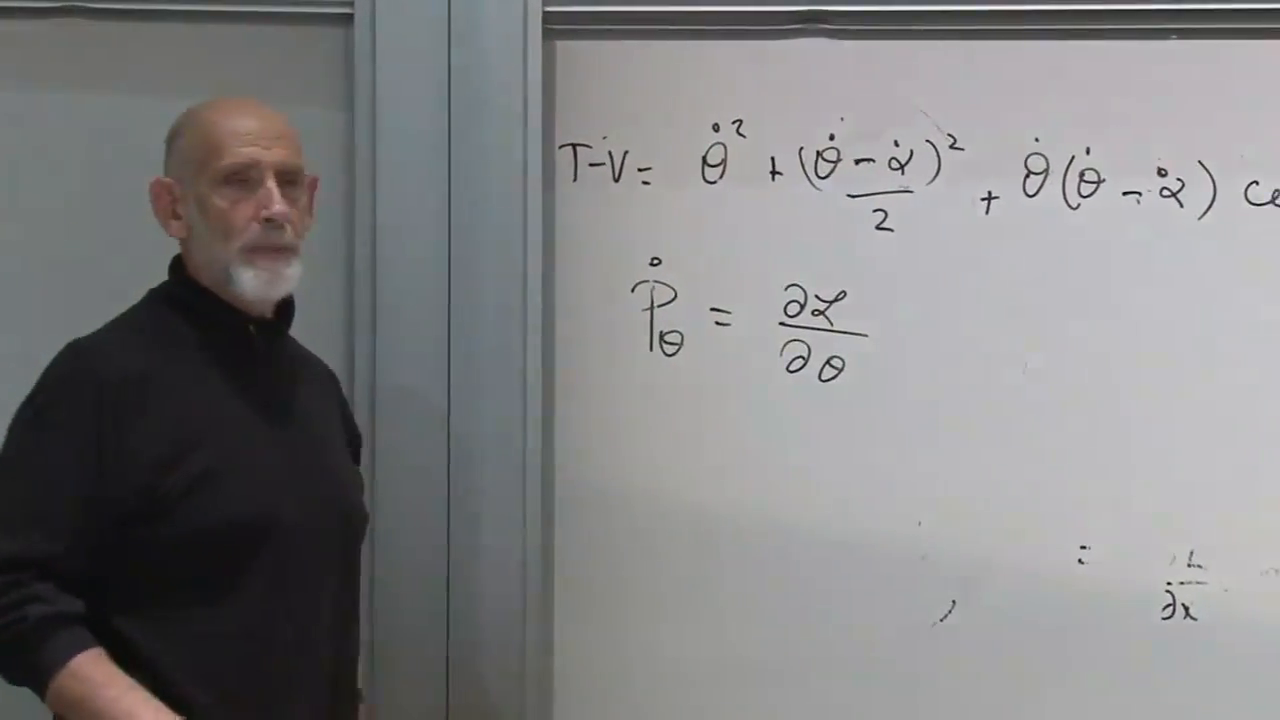
\includegraphics[width=0.84\textwidth]{lecture_06_figure_02.png}
  \caption{Le calcul du pendule sans gravité et \(\dot p_\theta=\partial L/\partial\theta\). La ligne supérieure du tableau conserve la notation locale dont les signes sont incohérents, évoquée dans la question ; la formule normalisée est donnée par l’équation ~\eqref{eq:l6-double-kinetic}.}
  \lectureframe{00:45:50}
\end{figure}

Une fois \(T\) et \(V\) connus, il ne reste qu’à obtenir les équations par dérivation. Les tensions des tiges et les forces qui imposent leur longueur fixe ont, là encore, disparu grâce au choix des coordonnées.

\subsection{Ce que la conservation implique ou n’implique pas}

\begin{classroomqa}
  \audiencequestion{Peut-on déterminer directement à partir des équations si le double pendule est chaotique ?
  \lecturetimestamp{00:44:57--00:45:25}}
  \lecturerresponse{En général, pas par une simple inspection. Quand les paramètres ou les énergies varient, un système peut passer d’un comportement régulier à un comportement chaotique. Ce sujet exige davantage que l’examen brut des équations et sera abordé plus loin.}
\end{classroomqa}

\begin{classroomqa}
  \audiencequestion{Dans un système conservatif, est-ce que chaque \(\dot p_i\) est nul ?
  \lecturetimestamp{00:45:25--00:46:24}}
  \lecturerresponse{Non. L’équation générale est
  \(\dot p_i=\partial L/\partial q_i\). Cette dérivée ne s’annule que si \(q_i\) est cyclique. Une coordonnée cyclique est le cas particulièrement simple où la symétrie se traduit par le déplacement d’une coordonnée tandis que les autres restent fixes.}
\end{classroomqa}

Si le seul objectif est de calculer l’évolution numérique, un système de coordonnées peu commode reste utilisable ; il produit simplement des équations plus longues. L’intérêt d’un choix judicieux est conceptuel : le moment conservé se voit avant même de résoudre les équations.

\begin{classroomqa}
  \audiencequestion{Sans gravité, un double pendule se comporte-t-il aussi simplement qu’un pendule libre unique ?
  \lecturetimestamp{00:47:02--00:47:35}}
  \lecturerresponse{Un rotor libre unique tourne uniformément, car son unique moment cinétique détermine son mouvement. Un double pendule peut présenter un mouvement relatif très complexe tout en conservant son moment cinétique total. Si les deux vitesses angulaires sont initialement nulles, le système reste au repos ; sinon, ses deux parties interagissent.}
\end{classroomqa}

\begin{classroomqa}
  \audiencequestion{En l’absence de gravité, \(\dot\theta\) et \(\dot\alpha\) sont-ils constants séparément ?
  \lecturetimestamp{00:47:36--00:52:42}}
  \lecturerresponse{Non. La conservation signifie \(\dot p_\theta=0\), et non \(\ddot\theta=0\) ou \(\ddot\alpha=0\). L’expression de \(p_\theta=\partial L/\partial\dot\theta\) dépend des deux vitesses angulaires et de \(\alpha\). Les tiges transmettent des couples, ce qui permet aux deux pendules d’échanger moment cinétique et énergie. C’est analogue à deux masses reliées par un ressort : la quantité de mouvement totale et la vitesse du centre de masse sont constantes, tandis que les vitesses individuelles oscillent. L’analogue rotationnel est une combinaison collective particulière, et non l’un ou l’autre angle pris séparément.}
\end{classroomqa}

\begin{classroomqa}
  \audiencequestion{Les forces qui échangent le moment cinétique sont-elles transmises par les tiges ?
  \lecturetimestamp{00:52:43--00:53:34}}
  \lecturerresponse{Oui. Une force transmise le long d’une tige n’est pas nécessairement dirigée vers le pivot de l’autre mouvement et peut donc exercer un couple. Un couple est simplement la tendance d’une force à produire une rotation ; ici, il entraîne des accélérations angulaires individuelles non nulles.}
\end{classroomqa}

\section{L’hamiltonien, troisième formulation}

L’hamiltonien est l’énergie, mais ce n’est là que sa première signification. Il est aussi au fondement d’une troisième formulation de la mécanique. Les équations de Newton utilisent les forces et les accélérations. Le principe de l’action stationnaire donne les équations d’Euler--Lagrange. Pour les systèmes réguliers, la mécanique hamiltonienne est équivalente à cette formulation, mais ses variables et sa géométrie sont différentes.

Au lieu de \(q_i\) et de \(\dot q_i\), utilisons \(q_i\) et leurs moments conjugués \(p_i\). Décrire l’état d’un système à \(n\) degrés de liberté exige \(2n\) nombres dans l’une ou l’autre formulation : positions et vitesses, ou positions et moments. Le lien entre ces descriptions est
\begin{equation}
  p_i=\frac{\partial L}{\partial\dot q_i}.
  \label{eq:l6-legendre-map}
\end{equation}
Lorsque ces relations peuvent être inversées pour exprimer les vitesses \(\dot q_i(q,p)\), on définit
\begin{equation}
  H(q,p)=\sum_i p_i\dot q_i-L(q,\dot q).
  \label{eq:l6-hamiltonian-definition}
\end{equation}
Les vitesses du membre de droite sont alors éliminées au profit de \(q\) et de \(p\). Cette inversibilité est l’hypothèse de régularité de la transformation de Legendre. Les lagrangiens singuliers exigent la théorie plus générale des contraintes ; cette construction élémentaire ne les traite pas.

\subsection{La réversibilité avant le calcul infinitésimal}

Considérons un ensemble fini d’états abstraits reliés par des flèches. Même une règle déterministe peut ne pas être réversible si deux états antérieurs aboutissent à un même état ultérieur. L’avenir est unique, mais le passé ne l’est pas. Inverser toutes les flèches produit le défaut opposé : un état se ramifie en plusieurs futurs. Dans le premier schéma, les flèches convergent ; dans le second, elles divergent.

\begin{figure}[htbp]
  \centering
  \includegraphics[width=0.86\textwidth]{lecture_06_figure_11.png}
  \caption{Applications d’états abstraits illustrant la différence entre des cycles réversibles et une convergence ou une divergence interdites.}
  \lectureframe{00:56:20}
\end{figure}

L’évolution hamiltonienne fournira la version continue de cet énoncé. Un nuage de points de l’espace des phases peut se déplacer et se déformer, mais il ne peut pas acquérir de puits qui efface les distinctions entre états, ni de source qui engendre plusieurs futurs à partir d’un seul état. La démonstration viendra plus tard ; pour l’instant, ces schémas motivent la géométrie.

\begin{classroomqa}
  \audiencequestion{Le schéma abstrait des états représente-t-il un objet qui se déplace dans un champ gravitationnel ?
  \lecturetimestamp{00:58:02--00:58:35}}
  \lecturerresponse{Non. Les points sont de simples états abstraits et les flèches définissent une règle de changement d’état. Aucune signification spatiale ou gravitationnelle n’a été attribuée au dessin.}
\end{classroomqa}

\begin{classroomqa}
  \audiencequestion{Comment distinguer une application d’états à convergence interdite d’un trou noir ?
  \lecturetimestamp{00:58:40--00:59:28}}
  \lecturerresponse{Ce n’est pas facile et la question est subtile. Elle est légitime, mais une réponse correcte exige de décrire soigneusement l’état complet et son évolution quantique et gravitationnelle. Le schéma élémentaire ne suffit pas à trancher.}
\end{classroomqa}

\section{Un oscillateur adapté à l’espace des phases}

Avant de dériver les équations générales, considérons un oscillateur harmonique écrit dans des variables délibérément adaptées :
\begin{equation}
  L=\frac{1}{2\omega}\dot q^2-\frac{\omega}{2}q^2.
  \label{eq:l6-rescaled-lagrangian}
\end{equation}
Son moment conjugué est
\begin{equation}
  p=\frac{\partial L}{\partial\dot q}=\frac{\dot q}{\omega},
  \qquad
  \dot q=\omega p.
  \label{eq:l6-rescaled-momentum}
\end{equation}
En substituant dans l’équation ~\eqref{eq:l6-hamiltonian-definition}, on obtient
\begin{align}
  H&=p\dot q-L\\
   &=\omega p^2-\frac{\omega p^2}{2}+\frac{\omega q^2}{2}
    =\frac{\omega}{2}(p^2+q^2).
  \label{eq:l6-oscillator-hamiltonian}
\end{align}

\begin{figure}[htbp]
  \centering
  \includegraphics[width=0.86\textwidth]{lecture_06_figure_12.png}
  \caption{Transformation de Legendre de l’oscillateur adapté et hamiltonien symétrique \(H=\tfrac{\omega}{2}(p^2+q^2)\).}
  \lectureframe{01:08:20}
\end{figure}

L’espace des \(q\) et \(p\) est l’espace des phases. Un degré de liberté donne un plan bidimensionnel ; deux degrés de liberté donnent un espace des phases à quatre dimensions. À énergie fixée pour l’oscillateur,
\begin{equation}
  p^2+q^2=\frac{2H}{\omega},
  \label{eq:l6-energy-circle}
\end{equation}
la trajectoire reste donc sur un cercle. La conservation de l’énergie confine le mouvement à une telle courbe.

\begin{figure}[htbp]
  \centering
  \includegraphics[width=0.82\textwidth]{lecture_06_figure_13.png}
  \caption{Cercles d’énergie constante emboîtés dans le plan des phases de l’oscillateur, avec \(q\) en abscisse et \(p\) en ordonnée.}
  \lectureframe{01:13:20}
\end{figure}

\section{Dérivation des équations de Hamilton}

La dérivation repose sur le calcul différentiel d’une fonction de plusieurs variables. Pour \(F(q,p)\),
\begin{equation}
  \delta F=\sum_i\left(
  \frac{\partial F}{\partial q_i}\delta q_i
  +\frac{\partial F}{\partial p_i}\delta p_i\right).
  \label{eq:l6-total-differential}
\end{equation}
On peut lire les coefficients dans les deux sens : le coefficient de \(\delta q_i\) est \(\partial F/\partial q_i\), et celui de \(\delta p_i\) est \(\partial F/\partial p_i\).

Faisons maintenant varier l’expression définissant \(H\) :
\begin{align}
  \delta H
  &=\sum_i\left(\dot q_i\,\delta p_i
       +p_i\,\delta\dot q_i\right)-\delta L\\
  &=\sum_i\left(\dot q_i\,\delta p_i
       +p_i\,\delta\dot q_i
       -\frac{\partial L}{\partial q_i}\delta q_i
       -\frac{\partial L}{\partial\dot q_i}\delta\dot q_i\right).
  \label{eq:l6-vary-hamiltonian}
\end{align}
Comme \(\partial L/\partial\dot q_i=p_i\), les deux termes \(\delta\dot q_i\) s’annulent. Les équations d’Euler--Lagrange donnent \(\partial L/\partial q_i=\dot p_i\), d’où
\begin{equation}
  \delta H=\sum_i\left(\dot q_i\,\delta p_i
                     -\dot p_i\,\delta q_i\right).
  \label{eq:l6-reduced-variation}
\end{equation}

\begin{figure}[htbp]
  \centering
  \includegraphics[width=0.86\textwidth]{lecture_06_figure_14.png}
  \caption{Développement de \(\delta H\) par la règle du produit avant l’annulation des termes \(p_i\,\delta\dot q_i\).}
  \lectureframe{01:18:40}
\end{figure}

En comparant l’équation ~\eqref{eq:l6-reduced-variation} à la différentielle générale de l’équation ~\eqref{eq:l6-total-differential}, l’identification des coefficients indépendants donne les équations de Hamilton :
\begin{equation}
  \boxed{
  \dot q_i=\frac{\partial H}{\partial p_i},
  \qquad
  \dot p_i=-\frac{\partial H}{\partial q_i}.}
  \label{eq:l6-hamilton-equations}
\end{equation}

\begin{figure}[htbp]
  \centering
  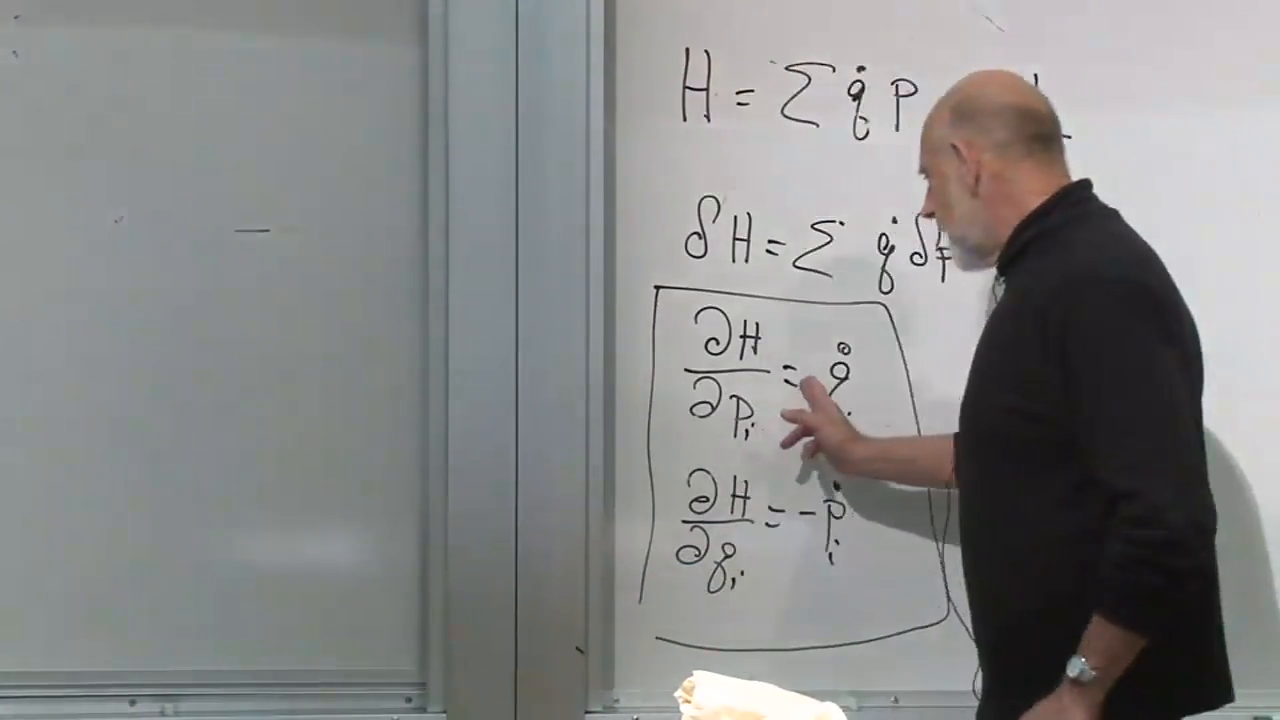
\includegraphics[width=0.78\textwidth]{lecture_06_figure_03.png}
  \caption{Définition de l’hamiltonien, sa variation et équations canoniques encadrées.}
  \lectureframe{01:22:18}
\end{figure}

Pour \(n\) coordonnées, ce sont \(2n\) équations du premier ordre. La formulation d’Euler--Lagrange fournit plutôt \(n\) équations du second ordre. La quantité de données initiales et le contenu physique sont identiques.

\section{Le mouvement de l’oscillateur comme rotation rigide}

En appliquant l’équation ~\eqref{eq:l6-hamilton-equations} à l’équation ~\eqref{eq:l6-oscillator-hamiltonian}, on obtient
\begin{equation}
  \dot q=\omega p,
  \qquad
  \dot p=-\omega q.
  \label{eq:l6-oscillator-first-order}
\end{equation}
En dérivant la première équation et en utilisant la seconde,
\begin{equation}
  \ddot q=\omega\dot p=-\omega^2q.
  \label{eq:l6-oscillator-second-order}
\end{equation}
Les deux équations du premier ordre sont donc exactement l’équation habituelle de l’oscillateur du second ordre, accompagnée de la définition du moment.

Dans l’espace des phases, le vecteur vitesse en \((q,p)\) est
\((\dot q,\dot p)=(\omega p,-\omega q)\), tangent au cercle d’énergie.
Tous les rayons tournent à la même vitesse angulaire \(\omega\). On peut imaginer le plan entier comme une hélice rigide ou comme un fluide fictif incompressible. Ses points circulent ; ils ne se contractent pas vers un puits et ne s’éloignent pas d’une source.

\begin{figure}[htbp]
  \centering
  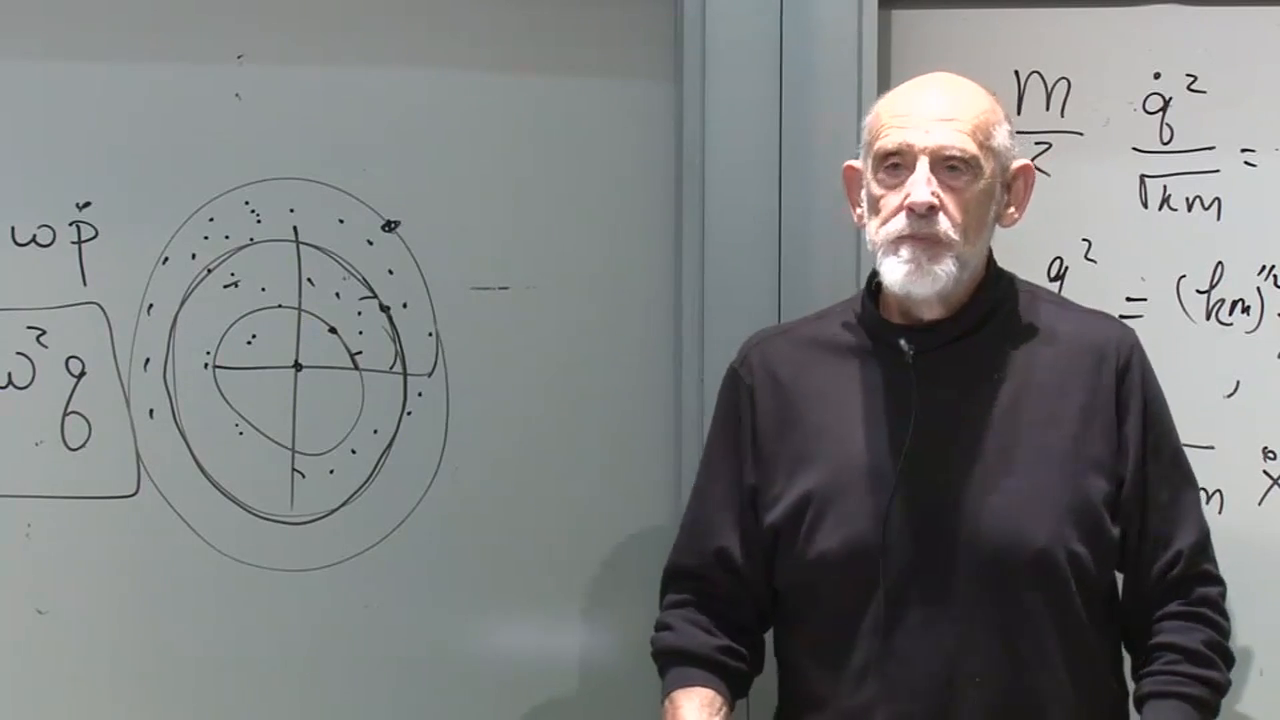
\includegraphics[width=0.86\textwidth]{lecture_06_figure_04.png}
  \caption{Nuage de points initiaux répartis sur des trajectoires emboîtées de l’espace des phases. L’évolution hamiltonienne déplace le nuage au lieu de le faire s’effondrer vers un état privilégié.}
  \lectureframe{01:39:27}
\end{figure}

\begin{figure}[htbp]
  \centering
  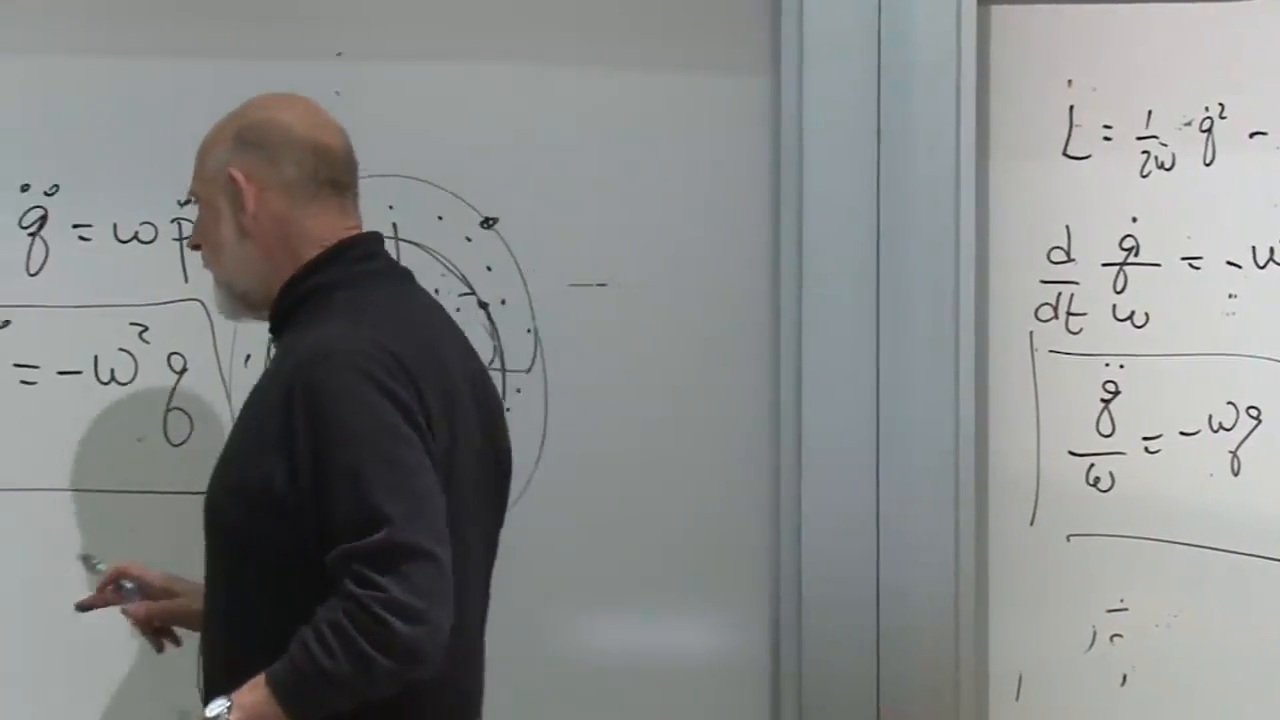
\includegraphics[width=0.90\textwidth]{lecture_06_figure_05.png}
  \caption{Portrait de phase de l’oscillateur, à côté de l’équation équivalente d’Euler--Lagrange
  \(\ddot q/\omega=-\omega q\).}
  \lectureframe{01:42:10}
\end{figure}

L’étape suivante consistera à transformer l’analogie du fluide en théorème : l’évolution hamiltonienne ne présente aucune convergence ni divergence locale. Ce résultat relie à nouveau la mécanique continue aux applications réversibles des états considérées au début du cours.

\section{Questions qui mettent en évidence le choix des coordonnées}

\begin{classroomqa}
  \audiencequestion{L’hypothèse selon laquelle on peut exprimer les vitesses en fonction de \(q\) et de \(p\) est-elle un théorème ou une propriété empirique des systèmes physiques ?
  \lecturetimestamp{01:29:08--01:29:45}}
  \lecturerresponse{Dans ce développement élémentaire, c’est une régularité empirique, qui trouve une motivation plus profonde en mécanique quantique. Plus précisément, la matrice jacobienne de l’équation ~\eqref{eq:l6-legendre-map} par rapport aux vitesses doit être non singulière. La mécanique moderne comprend aussi d’importants lagrangiens singuliers, notamment pour les systèmes contraints et de jauge, mais leur formulation hamiltonienne exige un traitement supplémentaire des contraintes.}
\end{classroomqa}

Une objection portant sur les unités explique pourquoi l’oscillateur a été écrit sous la forme inhabituelle de l’équation ~\eqref{eq:l6-rescaled-lagrangian}. Commençons plutôt par la coordonnée ordinaire \(x\) :
\begin{equation}
  L=\frac{m}{2}\dot x^2-\frac{k}{2}x^2,
  \qquad
  \omega=\sqrt{\frac{k}{m}}.
  \label{eq:l6-ordinary-oscillator}
\end{equation}
Choisissons
\begin{equation}
  q=(km)^{1/4}x.
  \label{eq:l6-oscillator-rescaling}
\end{equation}
On a alors \(q^2=\sqrt{km}\,x^2\) et
\(\dot q^2=\sqrt{km}\,\dot x^2\), ce qui transforme exactement l’équation ~\eqref{eq:l6-ordinary-oscillator} en l’équation ~\eqref{eq:l6-rescaled-lagrangian}. Le nouveau \(q\) est une coordonnée généralisée adaptée, et non une longueur ; son conjugué \(p\) n’est pas le moment mécanique ordinaire \(p_x=m\dot x\).

\begin{figure}[htbp]
  \centering
  \includegraphics[width=0.86\textwidth]{lecture_06_figure_15.png}
  \caption{Changement d’échelle dimensionnel de la coordonnée usuelle de l’oscillateur \(x\) vers la coordonnée adaptée \(q=(km)^{1/4}x\).}
  \lectureframe{01:36:10}
\end{figure}

\begin{classroomqa}
  \audiencequestion{Comment \(\omega p=\dot q\) peut-il être cohérent du point de vue dimensionnel, et pourquoi avoir choisi ces variables ?
  \lecturetimestamp{01:29:46--01:39:22}}
  \lecturerresponse{Le symbole \(q\) n’a pas nécessairement les dimensions d’une longueur, et son conjugué \(p\) n’a pas nécessairement les dimensions de \(m\dot x\). Le changement d’échelle de l’équation ~\eqref{eq:l6-oscillator-rescaling} préserve les dimensions du lagrangien et fait intervenir \(q\) et \(p\) de façon symétrique dans \(H\). Avec les variables d’origine,
  \[
    H=\frac{p_x^2}{2m}+\frac{kx^2}{2},
  \]
les courbes d’énergie constante dans le plan \((x,p_x)\) sont donc des ellipses. Dans le plan adapté \((q,p)\), ce sont des cercles. Le changement d’échelle a été choisi pour rendre cette symétrie visible.}
\end{classroomqa}

\begin{classroomqa}
  \audiencequestion{Comment des équations hamiltoniennes du premier ordre au nombre de \(2n\) peuvent-elles être équivalentes à des équations de Lagrange du second ordre au nombre de \(n\) ?
  \lecturetimestamp{01:39:24--01:42:30}}
  \lecturerresponse{Pour l’oscillateur, dérivons \(\dot q=\omega p\) et substituons \(\dot p=-\omega q\) ; on obtient le système \(\ddot q=-\omega^2q\). En partant directement du lagrangien, on trouve
  \[
    \frac{d}{dt}\left(\frac{\dot q}{\omega}\right)
      =-\omega q,
  \]
qui est la même équation du second ordre. On peut considérer qu’une équation de Hamilton définit le moment à partir de la vitesse, tandis que l’autre décrit l’évolution de ce moment.}
\end{classroomqa}

\section{Pourquoi l’espace des phases et l’énergie potentielle sont importants}

\begin{classroomqa}
  \audiencequestion{La puissance de la formulation hamiltonienne signifie-t-elle que l’espace des phases constitue une meilleure représentation géométrique que l’espace des configurations ?
  \lecturetimestamp{01:42:33--01:44:38}}
  \lecturerresponse{Ces deux espaces ont des fonctions différentes. L’espace des phases rend particulièrement visibles les cycles, les surfaces d’énergie constante et l’absence de convergence ou de divergence. Pour d’autres questions, l’espace des configurations peut être préférable. Si l’on insiste sur \(H\), c’est pour une raison plus profonde : cette quantité devient un objet central et plus intuitif en mécanique quantique, l’un des sujets modernes vers lesquels cette étude de la mécanique nous conduit.}
\end{classroomqa}

\begin{classroomqa}
  \audiencequestion{Faut-il considérer l’énergie potentielle comme l’intégrale de la force ?
  \lecturetimestamp{01:44:40--01:45:45}}
  \lecturerresponse{Pour les forces conservatives, cette affirmation est valable, à une constante près et avec le signe approprié. Il est plus utile de considérer le potentiel comme fondamental et d’en déduire la force généralisée :
  \[
    F_i=-\frac{\partial V}{\partial q_i}.
  \]
C’est précisément le terme qui apparaît dans \(\dot p_i=\partial L/\partial q_i\) lorsque \(L=T-V\) et que l’énergie cinétique ne dépend pas explicitement de \(q_i\).}
\end{classroomqa}

\begin{classroomqa}
  \audiencequestion{Quels problèmes de pointe cette voie vers la physique moderne est-elle censée éclairer ?
  \lecturetimestamp{01:45:46--01:47:47}}
  \lecturerresponse{Cette voie mène à la gravitation quantique et à la cosmologie ; à la physique des particules élémentaires, notamment au secteur de Higgs et aux neutrinos ; à la relativité ; à la théorie des cordes ; et à la théorie quantique des champs. Le problème théorique de fond reste de réunir ces éléments dans une structure cohérente, en particulier la mécanique quantique avec la gravitation, et la cosmologie avec la physique des particules. Il s’agissait d’un état des lieux des questions de pointe tel qu’il se présentait en 2011, et non de prétendre que leur solution était déjà connue.}
\end{classroomqa}

Les deux exemples avec contraintes et l’oscillateur s’inscrivent maintenant dans un même tableau. Les coordonnées généralisées éliminent les forces superflues. La symétrie sélectionne les moments canoniques conservés. La transformation de Legendre échange les vitesses contre les moments, et les équations de Hamilton décrivent la dynamique comme un flot dans l’espace des phases. Pour l’oscillateur, ce flot est une rotation rigide ; dans un système général, sa géométrie donnera un sens continu précis au mouvement réversible.